\subsection{Rewording at scale: machine paraphrases of 700 real tasks}
\label{sec:paraphrase}

The definitions of the \WidenTasksAll{} real tasks of Section~\ref{sec:many} were paraphrased by machine: back-translation through German and through French, sentence by sentence, with MarianMT models \citep{junczys2018marian,tiedemann2020opusmt} and beam search without sampling. On average \WidenKeptDe{}\% (German) and \WidenKeptFr{}\% (French) of the words of a definition survive; \WidenSameDe{} German and \WidenSameFr{} French paraphrases equal the original. Spanish and Italian pivots were made later, for the checks below (\WidenSpKept{}\% and \RerouteItKept{}\% of the words survive; \WidenSpSame{} and \RerouteItSame{} paraphrases equal the original). All paraphrases are used as they come. A paraphrased input is an input of its task with its definition replaced by the paraphrase. \WidenTasksCal{} tasks are kept for choosing and calibrating (not used again), \WidenTasksEval{} are used for evaluation in a random order of arrival, each with its zone. Nothing is trained: the tests compute routes only, with the T5-base word-vectors and the rule of Section~\ref{sec:method} unchanged. The tasks come from one collection, many of them are siblings, and the paraphrases are made by translation models, not by people; one split and one order of arrival are used except where stated.

\paragraph{Measures.} All are shares. \textsf{C}: tasks that arrive with at least one unedited input inside an older zone. \textsf{U}: unedited inputs given to their own task. \textsf{P}: paraphrased inputs inside their own task's zone and given to it (a correct certificate). \textsf{M}: paraphrased inputs certified for \emph{another} task (a wrong certificate: the answer is stable but comes from the wrong adapters). \textsf{R}: paraphrased inputs given to their own task, with or without a certificate. The letters name measures in this section and its appendix only; they are not the covariance, the radius or the zone of the method.

\paragraph{Result for \cert{}.} Tables~\ref{tab:widenmain} and~\ref{tab:widenspanish} give the numbers by pivot. With \WidenParaInputs{} paraphrased inputs (German and French together) \textsf{C}~=~\WidenRefTfiveC{}\%, \textsf{U}~=~\WidenRefTfiveU{}\%, \textsf{P}~=~\WidenRefTfiveP{}\%, \textsf{M}~=~\WidenRefTfiveM{}\% and \textsf{R}~=~\WidenRefTfiveR{}\%; across the pivots \textsf{P} runs from \WidenRefTfivePLow{}\% to \WidenRefTfivePHigh{}\%. On the Italian pivot (not in these tables) \textsf{P}~=~\WidenRefTfiveItP{}\%, \textsf{M}~=~\WidenRefTfiveItM{}\% and \textsf{R}~=~\WidenRefTfiveItR{}\%, in the same ranges. \cert{} was not tuned on any pivot. So between four and five in ten paraphrased inputs get a correct certificate, at most about one in ten a wrong one, the rest none, and about three quarters reach their own task. The \FiveCertRightLight{}\%, \FiveCertRightMedium{}\% and \FiveCertRightHeavy{}\% of Section~\ref{sec:reworded} were measured on five tasks far apart with the development rewordings. This is a limitation of the method as built: the zones are narrow at scale.

\paragraph{Can the zones be made wider?} Five attempts, each with a line fixed before the run (set-ups and numbers in Appendix~\ref{app:widen}; Table~\ref{tab:widenmain}, Figure~\ref{fig:widen}). None met its line.
(1) Hidden states of a frozen causal language model instead of word-vectors: line, 20 points more correct certificates at no higher collision rate and no more wrong certificates; verdict, against (wrong certificates rose).
(2) A metric in units of what paraphrasing does: line, 20 points more \textsf{P} at equal \textsf{C} with no more \textsf{M}; verdict, against.
(3) A frozen sentence encoder \citep{reimers2019sbert,wang2020minilm} with a split-conformal radius.
(4) A zone decided by a frozen inference model \citep{he2023debertav3} that judges whether two instructions ask for the same thing.
(5) The same judge, sentence by sentence.
For (3) to (5) the line was \textsf{P}~$\ge$~75\%, \textsf{M}~$\le$~5\% and \textsf{C}~$\le$~19\% (against: \textsf{P}~$<$~55\%, \textsf{M}~$>$~9\% or \textsf{C}~$>$~25\%), read on the French pivot for (3) and (4) and on the Italian pivot, which no study had read, for (5). Verdict: against for all three. (3) and (5) lift \textsf{P} but \textsf{M} stays above 9\% ((5), with \textsf{P} and \textsf{C} on the right side of the success lines, is the best point so far); (4) has far more wrong certificates and collisions (\textsf{M} far above 9\%, \textsf{C} above 25\%, \textsf{P} below 75\%; Table~\ref{tab:widenmain}). Most colliding tasks are siblings that differ in one or a few decisive words (a date format day-month against month-day, the closest integers against the farthest, a person's reaction against their intent in the ATOMIC tasks; Table~\ref{tab:widensiblings}), and every feature tried puts their rewordings together.

\begin{table}[t]
  \caption{Machine paraphrases of 700 real tasks, routes only: \cert{} and the attempts to widen the zones, in the setting named before each run. \textsf{C}, \textsf{P}, \textsf{M}, \textsf{R} in \%. ``Both'': German and French pivot together (\WidenParaInputs{} inputs); French rows \WidenParaInputsPivot{} inputs, except (4) and (5), which count one paraphrased instruction per task (\WidenTasksEval{}) and whose \textsf{C} is about the original instructions. Paper: T5-base word-vectors, $\kappa = 0.5$; its French row is the reference for (2) to (4). (1): SmolLM2-135M, last layer, one radius, own reference row. (2): metric fitted on paraphrases, read at the radius where \textsf{C} equals that of \cert{}; the pre-registered reference is the old ruler at that radius (\textsf{P} \WidenRulerTfivePOld{}\%, \textsf{M} \WidenRulerTfiveMOld{}\%). (3): MiniLM-L6, paraphrase ruler, $\alpha = 0.1$. (4): MiniLM filter and DeBERTa-v3-xsmall judge, $\tau = \WidenJudgeTau{}$. (5): the same judge sentence by sentence, Italian pivot.}
  \label{tab:widenmain}
  \centering
  \footnotesize
  \setlength{\tabcolsep}{3pt}
  \begin{tabular}{llcrrrrl}
    \toprule
    & Features and zone & Pivot & \textsf{C} & \textsf{P} & \textsf{M} & \textsf{R} & Verdict \\
    \midrule
    Paper & T5-base word-vectors, weighted mean & both & 16.9 & 40.5 & 7.6 & 75.4 & reference \\
    Paper & T5-base word-vectors, weighted mean & French & 16.9 & 39.8 & 9.2 & 75.4 & ref. for (2)--(4) \\
    \midrule
    (1) & SmolLM2 word-vectors & both & 18.9 & 42.1 & 8.9 & 75.6 & ref. for (1) \\
    (1) & SmolLM2 last layer & both & 25.7 & 64.9 & 13.7 & 83.2 & against \\
    (2) & T5-base, paraphrase ruler & French & 16.9 & 42.0 & 10.7 & 84.4 & against \\
    (3) & MiniLM, ruler, $\alpha = 0.1$ & French & 16.6 & 71.2 & 11.6 & 86.1 & against \\
    (4) & MiniLM and NLI judge & French & 36.0 & 58.9 & 34.7 & 64.7 & against \\
    (5) & MiniLM, sentence-wise NLI judge & Italian & 12.4 & 76.1 & 10.9 & 88.7 & against \\
    \midrule
    Bar (3)--(5) & \multicolumn{2}{l}{fixed in advance} & $\le 19$ & $\ge 75$ & $\le 5$ & & \\
    \bottomrule
\end{tabular}

\end{table}

\begin{figure}[t]
  \centering
  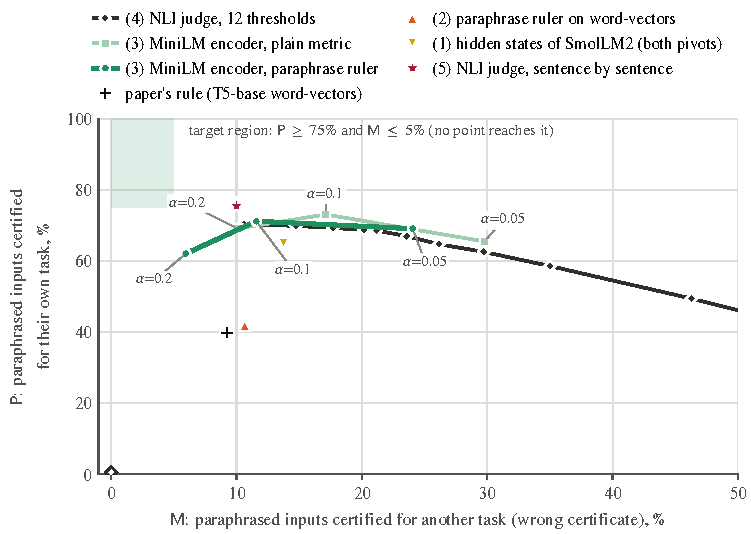
\includegraphics[width=0.86\linewidth]{figures/widen_tradeoff}
  \caption{Correct against wrong certificates on paraphrased inputs (French pivot; (1): both pivots). The shaded box is the target. The sentence encoder (3) is shown plain and with the ruler at $\alpha = 0.05, 0.1, 0.2$; the judge (4) has one point per threshold (the strictest, open, covers almost nothing; the loosest lies beyond the right edge). Only (3) at $\alpha = 0.1$, (4) at $\tau = \WidenJudgeTau{}$ and (5), at its French-pivot value, were named before the runs.}
  \label{fig:widen}
\end{figure}

\paragraph{A setting looked at after the runs.} The encoder with the ruler at $\alpha = 0.2$, not the primary setting, was ahead of \cert{} on every measure on the French pivot. Line fixed before the run: on Spanish-pivot paraphrases, which no study had read, with nothing fitted again, it gains at least \WidenSpAskP{} points in \textsf{P} and \WidenSpAskR{} in \textsf{R} with no more wrong certificates. Verdict: not confirmed (Table~\ref{tab:widenspanish}); the gain in \textsf{P} is \WidenSpGainP{} points, the gain in \textsf{R} (\WidenSpGainR{}) and \textsf{M} pass. On \WidenSplitCount{} other random splits (Table~\ref{tab:widensplits}) the encoder setting has more wrong certificates than \cert{} on \WidenSplitMoreM{} and more collisions on \WidenSplitMoreC{}: the advantage belongs to the original split. We report the encoder zone as a variant, not as an improvement. Its costs and the remaining numbers are in Appendix~\ref{app:widen}.

\begin{table}[t]
  \caption{Spanish-pivot check: \cert{} and the encoder setting (paraphrase ruler, $\alpha = 0.2$) on three pivots, \WidenSpInputs{} paraphrased inputs each; nothing fitted again for Spanish. In \%.}
  \label{tab:widenspanish}
  \centering
  \footnotesize
  \setlength{\tabcolsep}{3pt}
  \begin{tabular}{lrrrrrrrrrr}
    \toprule
    & & \multicolumn{3}{c}{French} & \multicolumn{3}{c}{German} & \multicolumn{3}{c}{Spanish} \\
    \cmidrule(lr){3-5} \cmidrule(lr){6-8} \cmidrule(lr){9-11}
    & \textsf{C} & \textsf{P} & \textsf{M} & \textsf{R} & \textsf{P} & \textsf{M} & \textsf{R} & \textsf{P} & \textsf{M} & \textsf{R} \\
    \midrule
    Paper's rule & 16.9 & 39.8 & 9.2 & 75.4 & 41.2 & 5.9 & 75.5 & 50.4 & 9.7 & 77.5 \\
    Encoder & 12.1 & 62.1 & 6.0 & 90.0 & 72.6 & 8.1 & 89.7 & 63.8 & 5.3 & 91.7 \\
    \bottomrule
\end{tabular}

\end{table}

\begin{table}[t]
  \caption{The same two rules on \WidenSplitCount{} other random splits of the \WidenTasksAll{} tasks, Spanish pivot: mean (smallest to largest), ruler and radius fitted again on each split. In \%.}
  \label{tab:widensplits}
  \centering
  \footnotesize
  \begin{tabular}{lcc}
    \toprule
    Spanish pivot & Paper's rule & Encoder \\
    \midrule
    Tasks that collide (\textsf{C}), \% $\downarrow$ & 16.0 (14.3 to 17.3) & 12.7 (9.1 to 16.6) \\
    Right certificate (\textsf{P}), \% $\uparrow$ & 49.4 (48.3 to 50.7) & 63.1 (55.5 to 70.0) \\
    Wrong certificate (\textsf{M}), \% $\downarrow$ & 7.9 (4.2 to 10.4) & 6.0 (2.4 to 9.7) \\
    Sent to own task (\textsf{R}), \% $\uparrow$ & 76.9 (75.8 to 78.1) & 90.4 (87.7 to 93.3) \\
    \bottomrule
\end{tabular}

\end{table}

\paragraph{Do later tasks re-route reworded inputs?} The paraphrased inputs show how often, among real tasks, a best-match rule changes an old route (Section~\ref{sec:stress} built such a case by hand). Each input's route right after its own task has arrived is compared with its route after all \WidenTasksEval{} tasks. Line fixed before the run (Appendix~\ref{app:reroute}): the zones add something at scale if \nearest{} changes at least 5\% of the routes and \cert{} at most half as many, and little if \nearest{} changes fewer than \RerouteLimitLow{}\%. Verdict: ``the zones add little here'' (Table~\ref{tab:reroute}). \nearest{} changed \RerouteNearNChanged{} of \RerouteInputs{} routes and \cert{} the same \RerouteCertNChanged{}, all outside every zone; none of the \RerouteCertInZone{}\% of inputs inside a zone at arrival changed, as Theorem~\ref{thm:writeonce} says, and the nearest-zone rule did not change them either. We had expected \RerouteExpectNearLow{}\% to \RerouteExpectNearHigh{}\% for \nearest{}; that was wrong. Here the certified switch adds the proof and no stability that we could measure.

\begin{table}[t]
  \caption{Do later tasks re-route reworded inputs? Routes only; \WidenTasksEval{} real tasks. ``Own'': share of the \RerouteInputs{} paraphrased inputs (French and German pivot) given to their own task after all tasks; ``Italian: own'': the same on the \RerouteInputsPivot{} Italian-pivot inputs. ``Changed'': route after all tasks differs from the route right after the input's own task arrived. ``In a zone'': inside a zone at arrival. ``Unedited'': unedited inputs given to their own task at the end (none changed under any rule). \signature{}: nearest signature in plain distance. \hybrid{}: oldest zone that holds the input, else \signature{}. \scaled{}: nearest signature with its distance divided by the distance of the task's signature to the nearest signature of the unrelated tasks. \certscaled{}: oldest zone that holds the input, else \scaled{}. \hybrid{} and \scaled{} were designed after the earlier results were seen, on the same data; none has a free setting.}
  \label{tab:reroute}
  \centering
  \scriptsize
  \setlength{\tabcolsep}{2pt}
  \begin{tabular}{lrrrrr}
    \toprule
    Rule & \shortstack[r]{Sent to own\\task, \% $\uparrow$} & \shortstack[r]{Italian pivot: sent\\to own task, \% $\uparrow$} & \shortstack[r]{Routes changed,\\\% (n) $\downarrow$} & \shortstack[r]{Inside a zone\\at arrival, \%} & \shortstack[r]{Unedited, sent to\\own task, \% $\uparrow$} \\
    \midrule
    \signature{} (plain nearest signature) & 91.3 & 93.1 & 2.22 (93) & -- & 98.4 \\
    \nearest{} (nearest zone) & 75.4 & 77.0 & 0.31 (13) & -- & 98.4 \\
    \cert{} (the rule of the paper) & 75.4 & 76.8 & 0.31 (13) & 48.1 & 83.1 \\
    \hybrid{} (zones, then nearest signature) & 85.6 & 88.5 & 1.95 (82) & 48.1 & 83.1 \\
    \scaled{} (scaled by the distance to unrelated text) & 94.4 & 95.9 & 1.60 (67) & -- & 98.4 \\
    \certscaled{} (zones, then \scaled{}) & 88.6 & 91.3 & 1.33 (56) & 48.1 & 83.1 \\
    \bottomrule
\end{tabular}

\end{table}

\begin{table}[t]
  \caption{The same rules on the benchmark tasks with the development rewordings (routes only): share of the \RerouteBenchInputs{} inputs given to their own task after the last task; ``(n)'': routes changed by later tasks (of \RerouteBenchInputs{}, including the inputs of the last task, which cannot change). With the original and the light wording every rule gives 100\% and changes nothing.}
  \label{tab:reroutebench}
  \centering
  \footnotesize
  \setlength{\tabcolsep}{3pt}
  \begin{tabular}{lrrrr}
    \toprule
    & \multicolumn{2}{c}{Five tasks} & \multicolumn{2}{c}{Fifteen tasks} \\
    \cmidrule(lr){2-3} \cmidrule(lr){4-5}
    Rule & \shortstack[r]{Medium wording:\\own task, \% $\uparrow$\\(routes changed)} & \shortstack[r]{Heavy wording:\\own task, \% $\uparrow$\\(routes changed)} & \shortstack[r]{Medium wording:\\own task, \% $\uparrow$\\(routes changed)} & \shortstack[r]{Heavy wording:\\own task, \% $\uparrow$\\(routes changed)} \\
    \midrule
    \signature{} & 76.8 (55) & 60.0 (100) & 71.6 (74) & 60.0 (100) \\
    \nearest{} & 100.0 (0) & 93.8 (0) & 100.0 (0) & 93.8 (0) \\
    \cert{} & 100.0 (0) & 93.8 (0) & 100.0 (0) & 93.8 (0) \\
    \hybrid{} & 76.8 (55) & 60.0 (100) & 71.6 (74) & 60.0 (100) \\
    \scaled{} & 100.0 (0) & 93.8 (0) & 100.0 (0) & 93.8 (0) \\
    \certscaled{} & 100.0 (0) & 93.8 (0) & 100.0 (0) & 93.8 (0) \\
    \bottomrule
\end{tabular}

\end{table}

Two more rules were added after this result, each with its reading fixed before it was computed (details in Appendix~\ref{app:reroute}). The plain nearest signature changed \RerouteSigNChanged{} routes (``some'', below the 5\% expected) but gave \RerouteSigOwnEnd{}\% of paraphrased inputs to their own task against \RerouteCertOwnEnd{}\% for \cert{} and \nearest{}: at this scale the simplest rule serves reworded inputs better and pays with about two silent changes in a hundred. Dividing the distance by the radius, the fallback of \cert{} chosen on the benchmark tasks, keeps routes stable here and gives fewer inputs to their own task. \hybrid{} (zones, then the plain signature; designed after that result, on the same data) keeps every certificate and gives \RerouteHybOwnEnd{}\% to their own task with \RerouteHybChanged{}\% changed routes, but on the benchmark with heavy rewording far fewer than \cert{} (\RerouteHybBenchFiveHeavyOwn{}\% against \RerouteCertBenchFiveHeavyOwn{}\%; Table~\ref{tab:reroutebench}). The two fallbacks trade places between the tests, so \hybrid{} is not a repair.

Why (read from the numbers, not tested): the radius of a zone is half the distance to the nearest known signature, unrelated or earlier. With $U_k$ the distance to the nearest unrelated signature, the radius is half of $U_k$ for all five benchmark tasks and \RerouteBBenchFifteenCount{} of fifteen, but for only \RerouteBShare{}\% of the \WidenTasksEval{} real tasks; for the others an earlier sibling is nearer, the newer sibling's radius is tiny and its reworded inputs are turned away.

Two fallbacks were tested for this. Line fixed before the run, verdict at scale read on a fourth pivot, Italian, that no study had read: at least \RerouteLineHeavy{}\% of inputs to their own task under heavy and \RerouteLineMedium{}\% under medium rewording on the benchmark (five and fifteen tasks) and at least \RerouteLineItalian{}\% on Italian; heavy below \RerouteLineHeavyAgainst{}\% or Italian below \RerouteLineItalianAgainst{}\% counts against. Verdict: scaling by the length of the opening failed (\RerouteNormHeavyFive{}\% under heavy rewording, although \RerouteNormItOwn{}\% on Italian); scaling by $U_k$ alone, \scaled{}, succeeded: on the benchmark it equals \cert{} under heavy and medium rewording (Table~\ref{tab:reroutebench}), and on the real tasks it gives \RerouteBgItOwn{}\% (Italian) and \RerouteBgOwnEnd{}\% (French and German) to their own task (Table~\ref{tab:reroute}). With the zones in front (\certscaled{}: same certificates, same theorem) it gives \RerouteCertFourOwnEnd{}\%, where \cert{} gives \RerouteCertOwnEnd{}\%, and the benchmark routes are those of \cert{}, input by input at every scored point (\RerouteIdFiveLast{} differing routes in \RerouteIdFiveComparisons{} comparisons on five tasks; fifteen tasks: \RerouteIdFifteenLast{} after the last task, \RerouteIdFifteenScored{} at any scored point), so every GPU score of \cert{} and \nearest{} is also the score of the variant. Limits of this variant, found at the end of the work: it changes more routes after arrival than \cert{} (Table~\ref{tab:reroute}); in the stress test of Section~\ref{sec:stress} a look-alike with the light rewording as its definition takes \RerouteStressCertFourMedium{} (medium) and \RerouteStressCertFourHeavy{} (heavy) of \RerouteStressOld{} uncertified old inputs that \cert{} kept, and one with the medium rewording takes \RerouteStressMedCertFourHeavy{} heavy ones, where \cert{} loses \RerouteStressMedCertHeavy{}; no certified input changes; the zones cost \RerouteZonesCost{} points of right routes on Italian, \RerouteZonesCostFG{} on French and German and \RerouteZonesCostEs{} on Spanish against the best rule without zones and give a proof for about half of the inputs (\RerouteCertInZone{}\% at arrival). The benchmark rewordings are the development set, no GPU run was repeated with it, no rule here was run with trained answers, and \cert{} stays the zone rule of every GPU run with instructions.

\paragraph{The guarantee does not depend on the zone.} Theorem~\ref{thm:writeonce} needs only that the zone is a fixed set once its task has arrived and that membership is computed reproducibly from frozen parts (Remark~\ref{rem:otherzones}). It holds for every zone here as defined; for the judge zone as measured, which judges only the \WidenJudgeLimit{} nearest tasks, see Appendix~\ref{app:widen}. A certificate promises a stable answer, not the right task. The edit bound of Proposition~\ref{prop:edits} does not carry over, because it needs an average. The development rewordings of the five benchmark tasks move further than a back-translation: with the sentence encoder \WidenEncBenchMediumZone{}\% (medium) and \WidenEncBenchHeavyZone{}\% (heavy) of them lie inside their own zone, all still go to the right task.

\subsection{Zones from the inputs of a task: the first test without instructions}
\label{sec:noinstruction}

This is the first test of the rule of Section~\ref{sec:bound} (Theorem~\ref{thm:bound}): a zone built from the inputs of the task itself, sized on held-out inputs, so that for any model and any later tasks each input of the task changes its answer with probability at most a chosen level. It was run before the recogniser of Section~\ref{sec:recogniser} existed, and its two findings (blocked tasks, the need for a better feature) are why that recogniser was built. Pilot A computes routes only, on a CPU; Pilot B trains a small model.

\paragraph{Pilot A: routes.} \emph{Set-up (fixed in the plan before the run).} Official benchmark files, instances only, the definition is never read. Sequences: the 15 tasks of SuperNI order~1 (Section~\ref{sec:protocol}), the 15 tasks of the Long Sequence benchmark in its order~3, and both as one sequence of \BoundTasksBoth{} tasks. All training inputs of a task are used for its zone (the plan said 800; the largest file has \BoundTrainMax{}); the official test inputs, never used for a zone, give the measures, so the condition of the theorem (test inputs like training inputs) is assumed for the benchmark's own split and checked by the coverage line. The feature is the weighted, rescaled average of the T5-base word-vectors of all tokens (cut at 256), as in \centre{} (weights and rescaling from the dev files of ten Long Sequence tasks). The score $a_k(x)$ is the distance to the 10th nearest fit input of task $k$; a second score is the distance to the mean of the fit features. \BoundMCal{} training inputs are held out for calibration (half for the \BoundSmallTasks{} tasks with fewer than 400, a deviation from the plan forced by the data; the smallest file has \BoundSmallMin{}); $\beta = 0.05$ (0.1 and 0.2 also reported); $q_k$ is the split-conformal quantile of Section~\ref{sec:bound}. An input goes to the oldest zone that holds it, else to the task with the smallest score divided by its $q_k$. Measures, averaged over the tasks: covered (test inputs inside their own zone), blocked (inside the zone of an older task when their task arrives), own task (after the last task), changed (route after the last task differs from the route at arrival).

\emph{Lines fixed before the run.} (1) The claim: on each sequence the average share of changed routes is at most $\beta$ plus two standard errors and the average coverage at least $1 - \beta$ minus two standard errors; if not, the paper has to say that test inputs are not like training inputs on these files. (2) The use: ``works without instructions'' if on average at least \BoundLineOwn{}\% of test inputs go to their own task and at most \BoundLineBlock{}\% are blocked; ``does not'' if fewer than \BoundLineNotOwn{}\% go to their own task or more than \BoundLineNotBlock{}\% are blocked; otherwise partial.

\begin{table}[t]
  \caption{Pilot A, no instruction (routes only; $\beta = 0.05$; means over the tasks of a sequence, in \%). Covered: promised at least \BoundCovPromised{}\% on average. Changed: promised at most \BoundAlpha{}\%. Blocked, own task: as in the text. ``sentence enc.'': frozen all-MiniLM-L6-v2 on the instance text, mean pooling; ``word-vec.'': the word-vector feature. Scores: 10-NN, distance to the 10th nearest fit input; mean, distance to the mean of the fit inputs; ratio, defined in the text.}
  \label{tab:boundpilot}
  \centering
  \footnotesize
  \setlength{\tabcolsep}{3pt}
  \begin{tabular}{lllrrrr}
    \toprule
    Sequence & Feature & Score & Covered, \% & \shortstack[r]{Routes\\changed, \% $\downarrow$} & \shortstack[r]{Blocked inputs,\\\% $\downarrow$} & \shortstack[r]{Sent to own\\task, \% $\uparrow$} \\
    \midrule
    SuperNI (15) & word-vec. & 10-NN & 96.1 & 0.7 & 86.5 & 12.7 \\
    SuperNI (15) & word-vec. & mean & 95.7 & 0.5 & 86.4 & 12.9 \\
    SuperNI (15) & word-vec. & ratio & 94.3 & 0.0 & 65.5 & 33.7 \\
    SuperNI (15) & sentence enc. & 10-NN & 94.7 & 1.4 & 46.6 & 51.0 \\
    SuperNI (15) & sentence enc. & mean & 95.2 & 0.9 & 59.8 & 37.9 \\
    SuperNI (15) & sentence enc. & ratio & 95.9 & 1.8 & 39.9 & 58.0 \\
    \midrule
    Long (15) & word-vec. & 10-NN & 94.9 & 1.1 & 88.3 & 10.6 \\
    Long (15) & word-vec. & mean & 95.0 & 1.0 & 88.6 & 10.4 \\
    Long (15) & word-vec. & ratio & 94.3 & 1.1 & 81.0 & 17.8 \\
    Long (15) & sentence enc. & 10-NN & 93.7 & 3.0 & 53.2 & 43.5 \\
    Long (15) & sentence enc. & mean & 94.0 & 2.9 & 62.6 & 34.4 \\
    Long (15) & sentence enc. & ratio & 94.4 & 1.4 & 54.3 & 43.8 \\
    \midrule
    Both (30) & word-vec. & 10-NN & 95.5 & 0.5 & 93.2 & 6.3 \\
    Both (30) & word-vec. & mean & 95.4 & 0.7 & 93.2 & 6.2 \\
    Both (30) & word-vec. & ratio & 94.3 & 1.5 & 78.1 & 20.3 \\
    Both (30) & sentence enc. & 10-NN & 94.2 & 2.3 & 63.5 & 34.1 \\
    Both (30) & sentence enc. & mean & 94.6 & 1.9 & 75.2 & 22.8 \\
    Both (30) & sentence enc. & ratio & 95.2 & 1.5 & 62.6 & 35.7 \\
    \bottomrule
\end{tabular}

\end{table}

\emph{Verdict on (1): the claim holds} on all three sequences (Table~\ref{tab:boundpilot}): coverage is above the lines (\BoundSuperniCovLimit{}\%, \BoundLongCovLimit{}\%, \BoundBothCovLimit{}\%; \BoundBothWordKnnFiveCov{}\% on both together) and changed routes are below them (\BoundSuperniChangedLimit{}\%, \BoundLongChangedLimit{}\%, \BoundBothChangedLimit{}\%; \BoundBothWordKnnFiveChanged{}\% on both together). No test input inside its own zone at arrival changed, as Theorem~\ref{thm:writeonce} says. The mean score and the levels 0.1 and 0.2 agree (SuperNI: coverage \BoundSuperniWordKnnTenCov{}\% and \BoundSuperniWordKnnTwentyCov{}\%, changed \BoundSuperniWordKnnTenChanged{}\% and \BoundSuperniWordKnnTwentyChanged{}\% at levels 0.1 and 0.2).
\emph{Verdict on (2): the use fails.} On both sequences together \BoundBothWordKnnFiveBlocked{}\% of test inputs are blocked and only \BoundBothWordKnnFiveOwn{}\% reach their own task (Table~\ref{tab:boundpilot} for each sequence), far from the \BoundLineOwn{}\% and \BoundLineBlock{}\% asked for.

\emph{A second score, designed after the first failed} (a second attempt, not an independent test; same lines, no free setting): in this feature the inputs of other tasks are about as close as a task's own outliers, so, as for the fallback in Section~\ref{sec:paraphrase}, distance is measured in units of the distance to unrelated text, $a_k(x) = d_k(x) / d_0(x)$, with $d_0$ the distance to the 10th nearest input of a fixed pool of \BoundPool{} unrelated inputs (instances only; a few from each real task of Section~\ref{sec:many} not in the sequences; fixed before the first task; for the Long Sequence tasks the pool holds instances of other files built on the same datasets, such as Yelp, IMDB and MNLI, which were not removed).
Result (word-vector feature, every row of the table): changed routes stay within the \BoundAlpha{}\% allowed and coverage within the \BoundCovPromised{}\% promised on average, within two standard errors; the use fails in every row (far more than \BoundLineNotBlock{}\% blocked). The ratio helps: on SuperNI \BoundSuperniWordRatioFiveOwn{}\% reach their own task instead of \BoundSuperniWordKnnFiveOwn{}\%, and \BoundToldApartCount{} of the 15 tasks are told apart almost completely (at least \BoundToldApartMin{}\% of test inputs reach their own task): \texttt{\BoundToldApartNames{}}, the three summarisation tasks, the dialogue task and the reading-comprehension task. Nine tasks have at most 10\% of their test inputs given to themselves (\BoundNotApartNames{}), the short-input and question tasks among them, because their inputs lie inside older zones. With the frozen sentence encoder as the feature (all-MiniLM-L6-v2 on the instance text, mean pooling; rows ``sentence enc.'' of Table~\ref{tab:boundpilot}) the claim holds again (coverage \BoundMiniCovLow{}\% to \BoundMiniCovHigh{}\%, at most \BoundMiniChangedMax{}\% of the routes changed in any row) and the use still fails by the lines fixed in advance (with the ratio score \BoundSuperniMiniRatioFiveBlocked{}\%, \BoundLongMiniRatioFiveBlocked{}\% and \BoundBothMiniRatioFiveBlocked{}\% blocked on the three sequences), but the sentence encoder tells the tasks apart better than the word-vector average: on the SuperNI tasks \BoundSuperniMiniRatioFiveBlocked{}\% blocked instead of \BoundSuperniWordRatioFiveBlocked{}\% and \BoundSuperniMiniRatioFiveOwn{}\% of the test inputs given to their own task instead of \BoundSuperniWordRatioFiveOwn{}\%. It was the secondary feature of the plan, so it changes no verdict.


\paragraph{Pilot B: trained answers on a small model.} \emph{Set-up.} The stand-alone code (\texttt{certified\_switch/}) on \texttt{t5-small}, the five tasks of the paper, definition removed from every input, \BoundBTrain{} training and \BoundBTest{} test inputs per task, \BoundBEpochs{} epochs, one seed, a CPU, \BoundBCal{} calibration inputs per task, $\beta = 0.05$. Compared on the same adapters: all adapters on, and the zones with the plain or the ratio score. It is a demonstration, not a result about scale.
\emph{Line fixed before the first run:} ``works'' if with the zones at most 10\% of the \BoundBCompared{} answers to earlier tasks change and forgetting is at most 3 points, while with all adapters on more than half change; ``does not'' if more than 20\% change.

\begin{table}[t]
  \caption{Pilot B, \texttt{t5-small}, five tasks, no definition in any input, one seed. Rouge-L averages over the tasks: ``Learned'' right after each task was learned, ``End'' at the end; forgetting is the average over the first four tasks of the drop from learned to end, so it is not the difference of the two columns. ``Changed'': of the \BoundBCompared{} answers to test inputs of the first four tasks, those that differ at the end. ``Own task'': test inputs given to their own task after the last task. Last column: per task in order, test inputs inside the zone of an older task when the task arrives.}
  \label{tab:boundpilotb}
  \centering
  \footnotesize
  \setlength{\tabcolsep}{3pt}
  \begin{tabular}{lrrrrrl}
    \toprule
    Rule & \shortstack[r]{Score\\right after\\learning $\uparrow$} & Final score $\uparrow$ & \shortstack[r]{Forgetting\\(points) $\downarrow$} & \shortstack[r]{Answers\\changed $\downarrow$} & \shortstack[r]{Sent to own\\task, \% $\uparrow$} & Blocked (of 50) \\
    \midrule
    All adapters on & 64.4 & 9.6 & 68.4 & 200 of 200 & -- & -- \\
    Zones, plain score & 24.1 & 24.1 & 0.0 & 0 of 200 & 21 & 0, 48, 50, 47, 50 \\
    Zones, ratio score & 36.7 & 33.6 & 3.8 & 8 of 200 & 50 & 0, 0, 23, 48, 45 \\
    \bottomrule
\end{tabular}

\end{table}

\emph{First run (plain score).} Verdict: it met the line (no answer changed, \BoundBPlainChanged{} of \BoundBCompared{}, against all of them with all adapters on) but was empty: \BoundBPlainFirstTrainBlocked{} of the \BoundBTrain{} training inputs of the second task lie inside the zone of the first, nearly all inputs of later tasks do too, only the first task was learned, and there was nothing to forget. The line had been badly chosen; before the second run was read it was corrected so that ``works'' also needs the tasks to be learned (average score right after learning at least 90\% of that with all adapters on) and at least 80\% of test inputs to reach their own task (other conditions as before: at most 20 of the \BoundBCompared{} answers changed, more than 100 with all adapters on, forgetting at most 3 points).
\emph{Second run (ratio score).} \BoundBRatioChanged{} of \BoundBCompared{} answers changed (4\%, where 5\% is allowed on average) and none of the \BoundBRatioInside{} test inputs inside their own zone changed; forgetting is \BoundBRatioFT{} points, above the 3 allowed; the tasks are not learned (\BoundBRatioLearned{} against \BoundBAllLearned{} with all adapters on, \BoundBRatioRatioToAll{}\%): only the first two tasks reach their all-adapters score (\BoundBRatioScoreOne{} and \BoundBRatioScoreTwo{}, the latter at the level of guessing under both rules), the third \BoundBRatioScoreThree{} against \BoundBAllScoreThree{}, the fourth and fifth \BoundBRatioScoreFour{} and \BoundBRatioScoreFive{} against \BoundBAllScoreFour{} and \BoundBAllScoreFive{}; only about \BoundBRatioOwn{}\% of test inputs reach their own task. Verdict by the corrected line: it does not work. The bound held in both runs. Without its definition the small model reached only the level of guessing (\BoundBAllGuessScore{}) on \BoundBAllGuess{} of the five tasks even with all adapters on; whether these tasks are learned better with their definition was not compared task by task.

\paragraph{What this subsection shows.} Reached: a guarantee that needs no instruction, is more than ``inside a zone nothing changes'' (each input changes its answer with probability at most a chosen level, for any model and any later tasks), is proved (Theorem~\ref{thm:bound}), and was met in every run (routes on 30 benchmark tasks; answers of a small model). Not reached: a method that works without instructions. With frozen word-vector features the zones of early tasks hold the inputs of later tasks; this is reported when a task arrives, but those tasks are then not learned, and no GPU run was made, because no pilot worked. The difficulty is now one thing: a frozen feature in which inputs of different tasks are apart without an instruction. A sentence encoder helps but does not suffice (\BoundBothMiniRatioFiveBlocked{}\% blocked at best on all 30 tasks); the hidden states of the frozen model are the feature of the recogniser of Section~\ref{sec:recogniser}, which needs no zone and blocks no task. The test inputs here are like the training inputs; a reworded or shifted input has no guarantee from this theorem.
